\chapter{Конструкторская часть}

В данном разделе будут представлены схемы алгоритмов вычисления расстояний Левенштейна и Дамерау-Левенштейна. Будут описаны типы и структуры данных, используемые для реализации, а также структура разрабатываемого программного обеспечения, оценено использование памяти. Кроме того будут выделены классы эквивалентности для тестирования.

\section{Разработка алгоритмов}

Схемы рекурсивного и матричного алгоритмов поиска расстояния Левенштейна представлены на рисунках \ref{img:recursive}-\ref{img:matrix} соответственно. Для алгоритма с использованием матрицы на рисунке \ref{img:recursion} приведена схема рекурсивной части, схема всего алгоритма - на рисунке \ref{img:cache}. Схема алгоритма Дамерау-Левенштейна приведена на рисунке \ref{img:dl}.

\begin{figure}[H]
	\begin{center}
		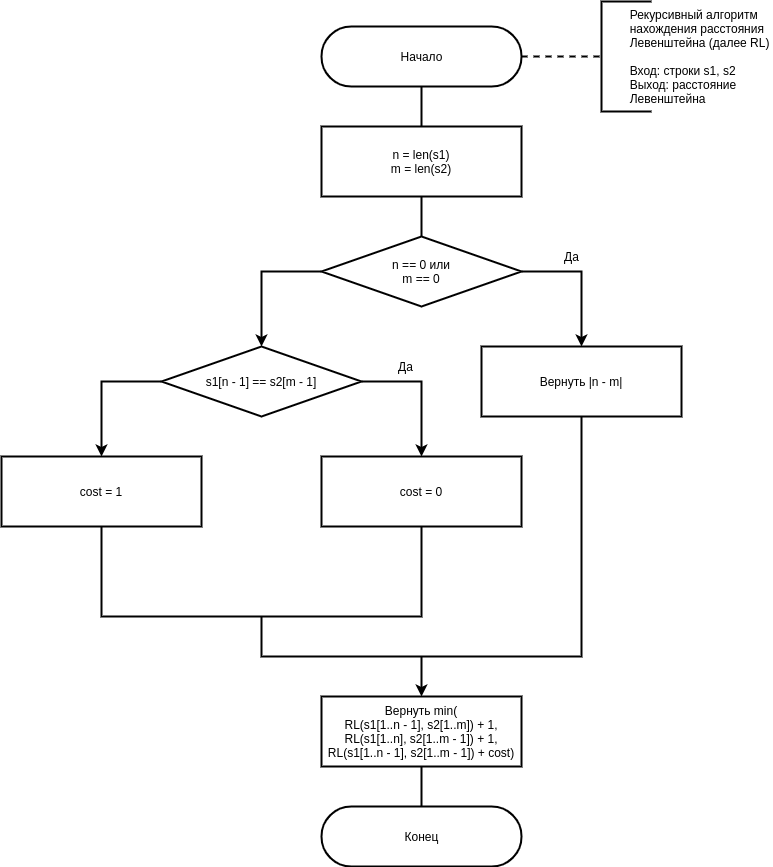
\includegraphics[scale=0.6]{img/recursive.png}
	\end{center}
	\captionsetup{justification=centering}
	\caption{Схема рекурсивного алгоритма нахождения расстояния Левенштейна}
	\label{img:recursive}
\end{figure}

\begin{figure}[H]
	\begin{center}
		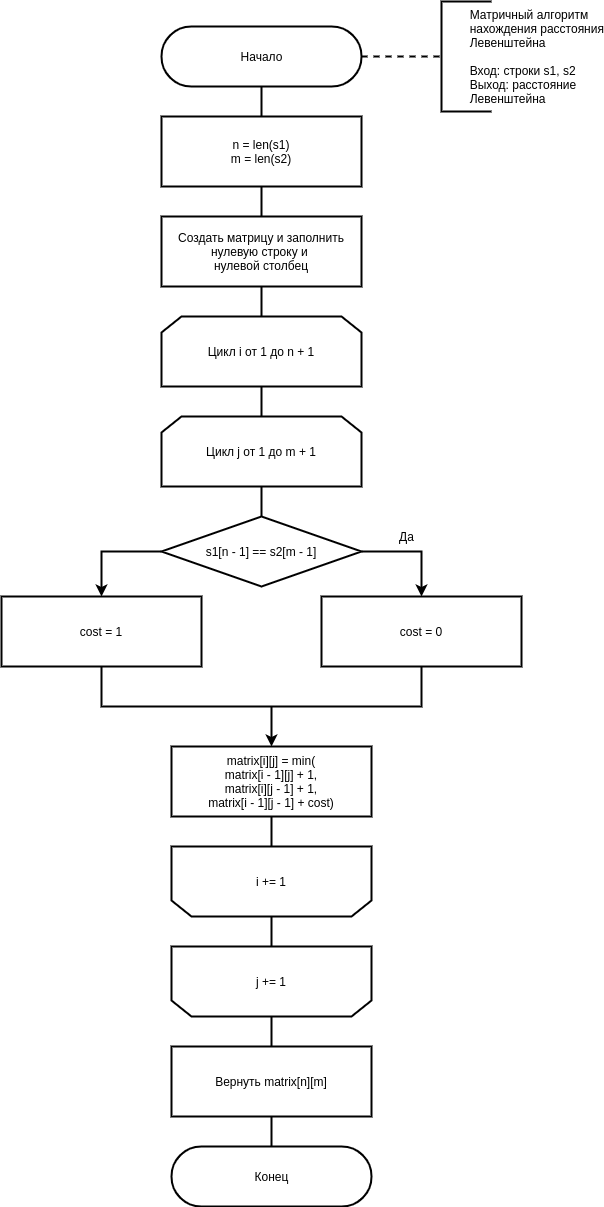
\includegraphics[scale=0.5]{img/matrix.png}
	\end{center}
	\captionsetup{justification=centering}
	\caption{Схема матричного алгоритма нахождения расстояния Левенштейна}
	\label{img:matrix}
\end{figure}

\begin{figure}[H]
	\begin{center}
		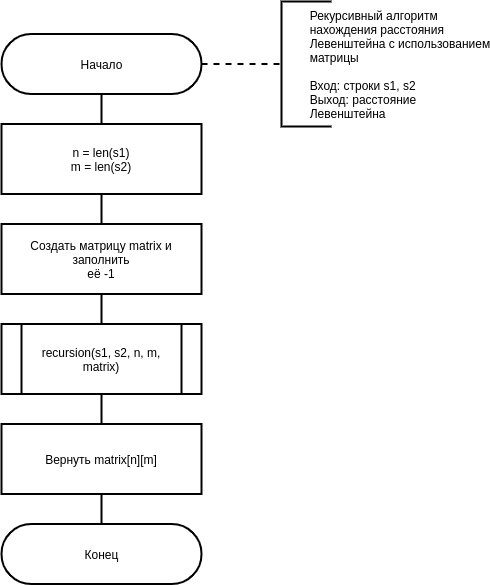
\includegraphics[scale=0.6]{img/cache.png}
	\end{center}
	\captionsetup{justification=centering}
	\caption{Схема алгоритма нахождения расстояния Левенштейна с использованием матрицы}
	\label{img:cache}
\end{figure}

\begin{figure}[H]
	\begin{center}
		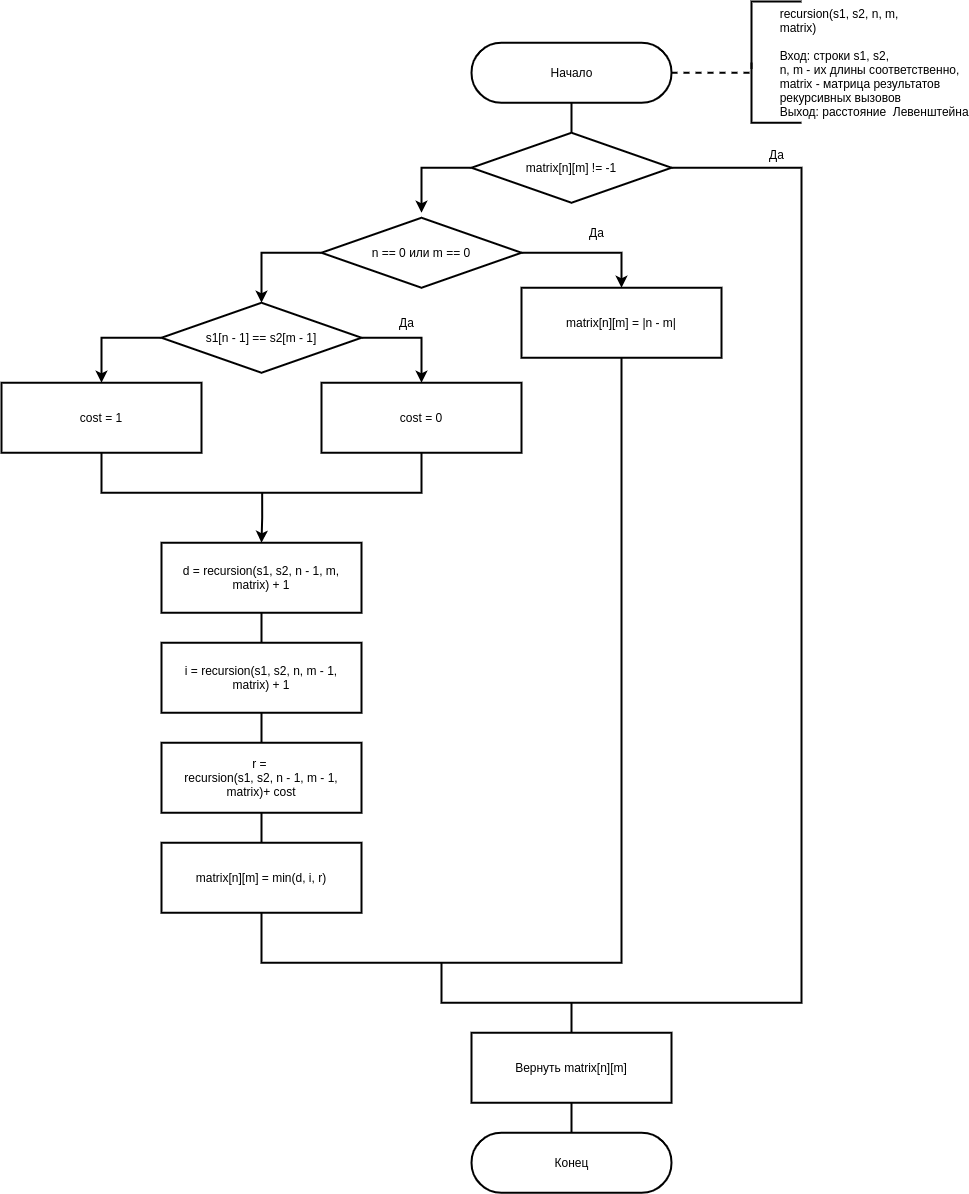
\includegraphics[scale=0.5]{img/recursion.png}
	\end{center}
	\captionsetup{justification=centering}
	\caption{Схема рекурсивной части алгоритма нахождения расстояния Левенштейна с использованием матрицы}
	\label{img:recursion}
\end{figure}

\begin{figure}[H]
	\begin{center}
		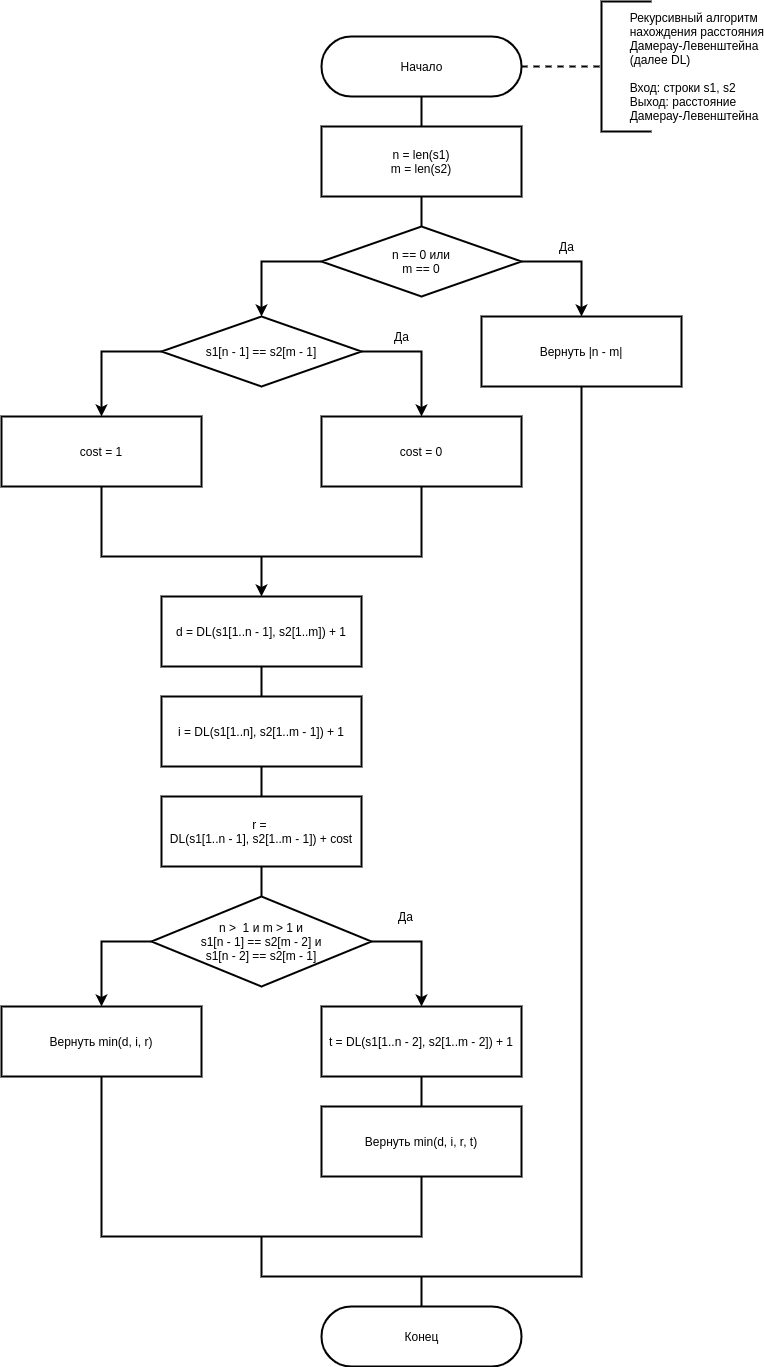
\includegraphics[scale=0.5]{img/dl.png}
	\end{center}
	\captionsetup{justification=centering}
	\caption{Схема рекурсивного алгоритма нахождения расстояния Дамерау-Левенштейна}
	\label{img:dl}
\end{figure}

\section{Описание используемых типов и структур данных}

Для реализации рассмотренных алгоритмов будут использованы следующие типы данных:

\begin{itemize}
	\item $str$ - для двух строк, поданных на вход;
	\item $int$ - для длин каждой из строк, поданных на вход, и для возвращаемого значения искомого расстояния.
\end{itemize}

Для реализации матричной версии алгоритма нахождения расстояния Левенштейна и версии с использованием матрицы используется двумерный список значений типа $int$.

\section{Использование памяти}

Алгоритм нахождения расстояния Дамерау-Левенштейна отличается от алгоритма нахождения расстояния Левенштейна добавлением операции транспозиции, что не влияет на объем используемой памяти. Поэтому проведем анализ используемой памяти для рекурсивного и нерекурсивного версий алгоритма Левенштейна.

Для рекурсивной версии при каждом вызове происходит выделение памяти под:

\begin{itemize}
	\item 2 строки типа $str$;
	\item 2 длины строк типа $int$;
	\item возвращаемое значение типа $int$;
	\item адрес возврата типа $int$;
	\item локальная переменная типа $int$.
\end{itemize}

При этом глубина рекурсии равна сумме длин двух строк. Таким образом, используемая память рекурсивной версии равна:

\begin{equation}
	\label{eq:rm}
	M_{r} = (5 \cdot sizeof(int)+2 \cdot sizeof(str))\cdot(|s1|+|s2|)
\end{equation}

Для нерекурсивной версии происходит выделение памяти под:

\begin{itemize}
	\item 2 строки типа $str$;
	\item 2 длины строк типа $int$;
	\item матрицу с размерами, равными длинам строк, увеличенным на 1;
	\item возвращаемое значение типа $int$;
	\item адрес возврата типа $int$;
	\item 5 локальных переменных типа $int$.
\end{itemize}

Таким образом, используемая память нерекурсивной версии равна:

\begin{equation}
	\label{eq:mm}
	M_{m} = (9+(|s1|+1) \cdot (|s2|+1)) \cdot sizeof(int)+2 \cdot sizeof(str)
\end{equation}

\section{Структура разрабатываемого ПО}

Программа состоит из следующих модулей:

\begin{itemize}
	\item main.py - главный файл программы, предоставляющий пользователю меня для выполнения основных функций;
	\item distances.py - файл, содержащий алгоритмы нахождения редакционного расстояния;
	\item str.py - файл, содержащий функции работы со строками;
	\item matrix.py - файл, содержащий функции работы с матрицами;
	\item time\_test.py - файл, содержащий функции замеров времени работы указанных алгоритмов;
	\item graph\_result.py - файл, содержащий функции визуализации временных характеристик описанных алгоритмов.
\end{itemize}

\section{Классы эквивалентности при тестировании}

Для тестирования разрабатываемой программы будут выделены следующие классы эквивалентности:

\begin{itemize}
	\item две пустые строки;
	\item одна пустая строка, одна нет;
	\item удаление/добавление символа в конец;
	\item удаление/добавление символа внутри строки;
	\item замена символов;
	\item транспозиция символов.
\end{itemize}

\section{Вывод}

Были представлены схемы алгоритмов вычисления расстояний Левенштейна и Дамерау-Левенштейна. Были указаны типы и структуры данных, используемые для реализации, и описана структура разрабатываемого программного обеспечения. Был проанализирован объем используемой памятия для рекурсивной и нерекурсивной версий алгоритмов. Также были выделены классы эквивалентности для тестирования ПО.
